\section{Three-level system}\label{sec:pw3l}

A two-level system is the simplest non-trivial quantum system and,
as seen in Sec.~\ref{sec:absorption+pw},
it is sufficient to illustrate
models of quantum time of arrival,
such as those based on complex potentials,
as well as relational models.
Therein, numerical examples have been shown, where the two approaches
---discrete Page--Wootters and the ``non Hermitian'' detector models---
lead to
compatible predictions.

A three-level atom (or a three-level quantum system in general) appears
naturally
as
the next computational step;
but far from being merely another excercise
---just at a slightly higher level of complexity
but otherwise showing, essentially, the same physics---
it is in fact the \emph{minimal} system \emph{required}
to realize a broad
phenomenology that includes the
\term{Stimulated Raman adiabatic passage}
---STIRAP \parencite{Ruschhaupt_AtomDiode, NonHermitianShortcutSTIRAP, OptimizedTransferSTIRAP, Ruschhaupt_STA23}
and the
\term{Electromagnetically induced transparency}
---EIT \parencite{EIT_Review}.

Also, it wil be shown that a three-level atom can model
a more robust and realistic
detector for time-of-arrival measurement, compared to the one implemented
with a two-level atom (as introduced in Sec.~\ref{sec:hist:detect}).
The atom can be ``driven'' by a laser
from the ground state $\ket{0}$ into the excited state $\ket{2}$,
then decay into a metastable state $\ket{1}$ at an intermediate energy
(see the above references, although they might use a slightly different notation).
This prevents the atom from decaying again and altering the ``arrival'' detection.

As usual, we're going to set $\hbar = 1$ in the following numerical computation,
based, once again, on the
\emph{NumPy} framework \parencite{comp:numpy},
within a
\term{Jupyter notebook} \parencite{comp:jupyter}.
Details can be consulted in the Appendix~\ref{detector-model-3-level-system}.
Full source code is available from the repository at ref. \cite{OwnJupyterRepo}.

In our numerical example, the following
Hamiltonian is considered:
\begin{equation}
  H \repr \frac{1}{96} \mqty(
    -2  & 0 & 32  \\
     0  & 2 & 8   \\
    32  & 8 & 3
  )
  \text{,}
\end{equation}
with respect to the fiducial basis $\qty{\ket{0}, \ket{1}, \ket{2}}$.
Let also
the initial state be $\ket{\psi(0)} = \ket{0} \repr \mqty(1 \\ 0 \\ 0)$.

The system will evolve \emph{unitarily}, according to $\ket{\psi(t)} = \E^{-\iu H t} \ket{\psi(0)}$,
which is computed numerically:
\begin{lstlisting}[language=Python]
import numpy as np
from scipy.linalg import expm, norm

H = np.array([
  [-2,     0,      32],
  [0,      2,       8],
  [32,     8,       3]
], np.complex_) / 96

psi_0 = np.array([1, 0, 0], np.complex_)

def U(t):
    return expm(-1j*H*t)

def unitary_psi(t):
    return U(t) @ psi_0
\end{lstlisting}

We're interested in the probability of the system to be in $\ket{0}$, $\ket{1}$, or $\ket{2}$,
which is given by $\abs{\braket{0, 1, 2}{\psi(t)}}^2$:
\begin{lstlisting}[language=Python]
def prob(t):
  probabilities = [0, 0, 0]
  for i in 0, 1, 2:
      probabilities[i] = norm(unitary_psi(t)[i])**2
  return probabilities
\end{lstlisting}
Such probabilities over time are shown in Figure \ref{fig:3lev:probs}. 

\begin{figure}[h]
  \begin{subfigure}[b]{\textwidth}
    \centering
    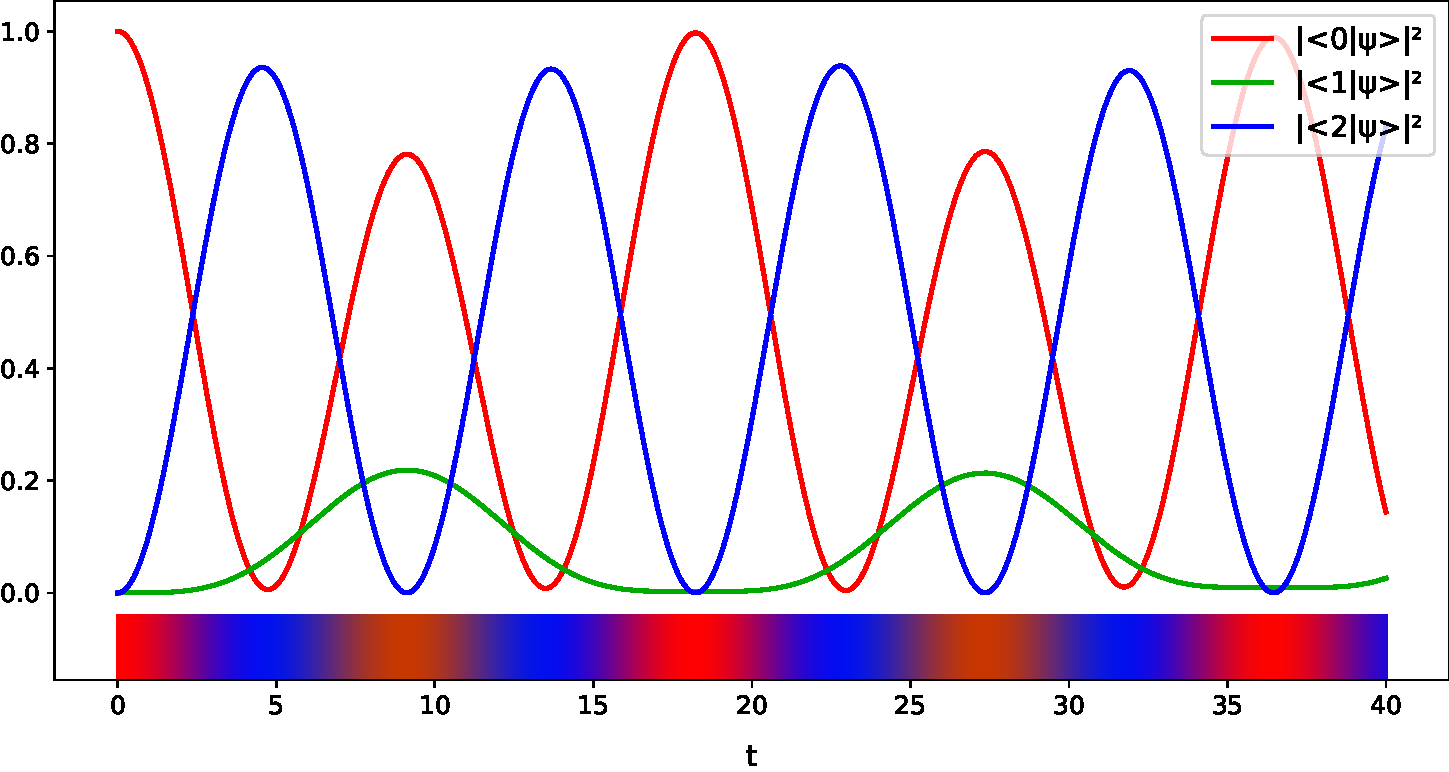
\includegraphics[width=.8\textwidth]{img/3ldetect/hermitian3lines.pdf}
    \subcaption{
      Probabilities for the three-level system.
      \emph{Note}:
        a three-level system allows a graphical representaion
        where primary colors can be combined
        (see the bar at the bottom) to immediately
        visualize which probability dominates.
    }
    \label{fig:3lev:probs:lines}
  \end{subfigure}
  \par\bigskip
  \par\bigskip
  \begin{subfigure}[b]{\textwidth}
    \centering
    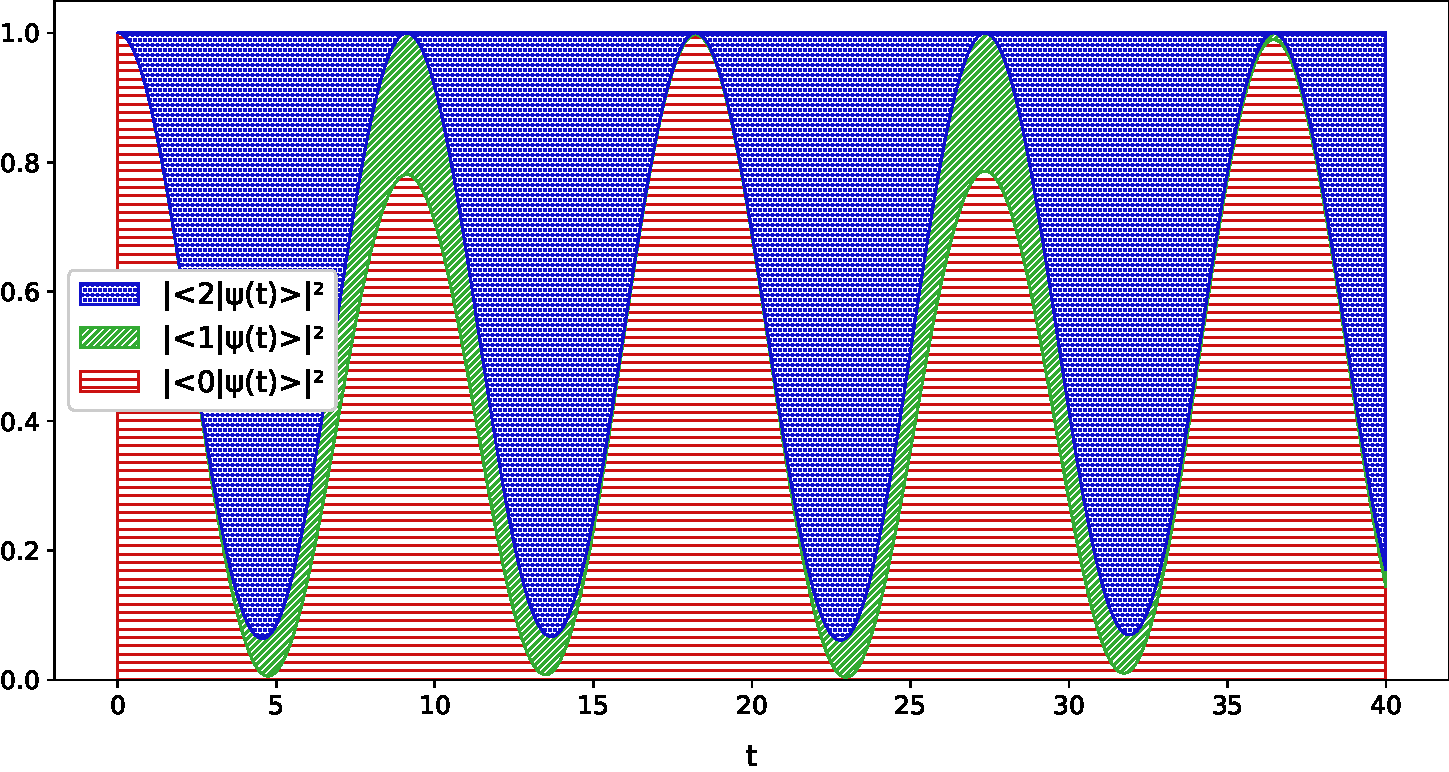
\includegraphics[width=.8\textwidth]{img/3ldetect/hermitian3color.pdf}
    \subcaption{\setstretch{1.25}
      \emph{Stacked} probability chart shows that their sum
      $\sum_{i=0}^{2} \abs{\braket{i}{\psi(t)}}^2$
      is constantly equal to 1 at any time $t$.
      That is equal to the norm $\norm{\psi(t)}^2$, which is indeed conserved
      as
      the system evolves \emph{unitarily}.
    }
    \label{fig:3lev:probs:stack}
  \end{subfigure}
  \par\bigskip
  \par\bigskip
  \caption{
    Probabilities
      $\abs{\braket{i}{\psi(t)}}^2$ for $i \in \qty{0, 1, 2}.$
  }
  \label{fig:3lev:probs}
\end{figure}

We are also interested in probability \term{amplitudes}:
complex values of
$\braket{0}{\psi(t)}$, 
$\braket{1}{\psi(t)}$, and
$\braket{2}{\psi(t)}$
are represented in the three-dimensional
plot in Fig.~\ref{fig:3lev:hermitianEvol}.
Once again, the two horizontal axes are used for the real and imaginary part of
$\braket{0, 1, 2}{\psi(t)}$,
while the independend variable $t$ (time) is represented on the vertical axis.
\begin{figure}[h]
  \begin{subfigure}[t]{\textwidth}
    \centering
    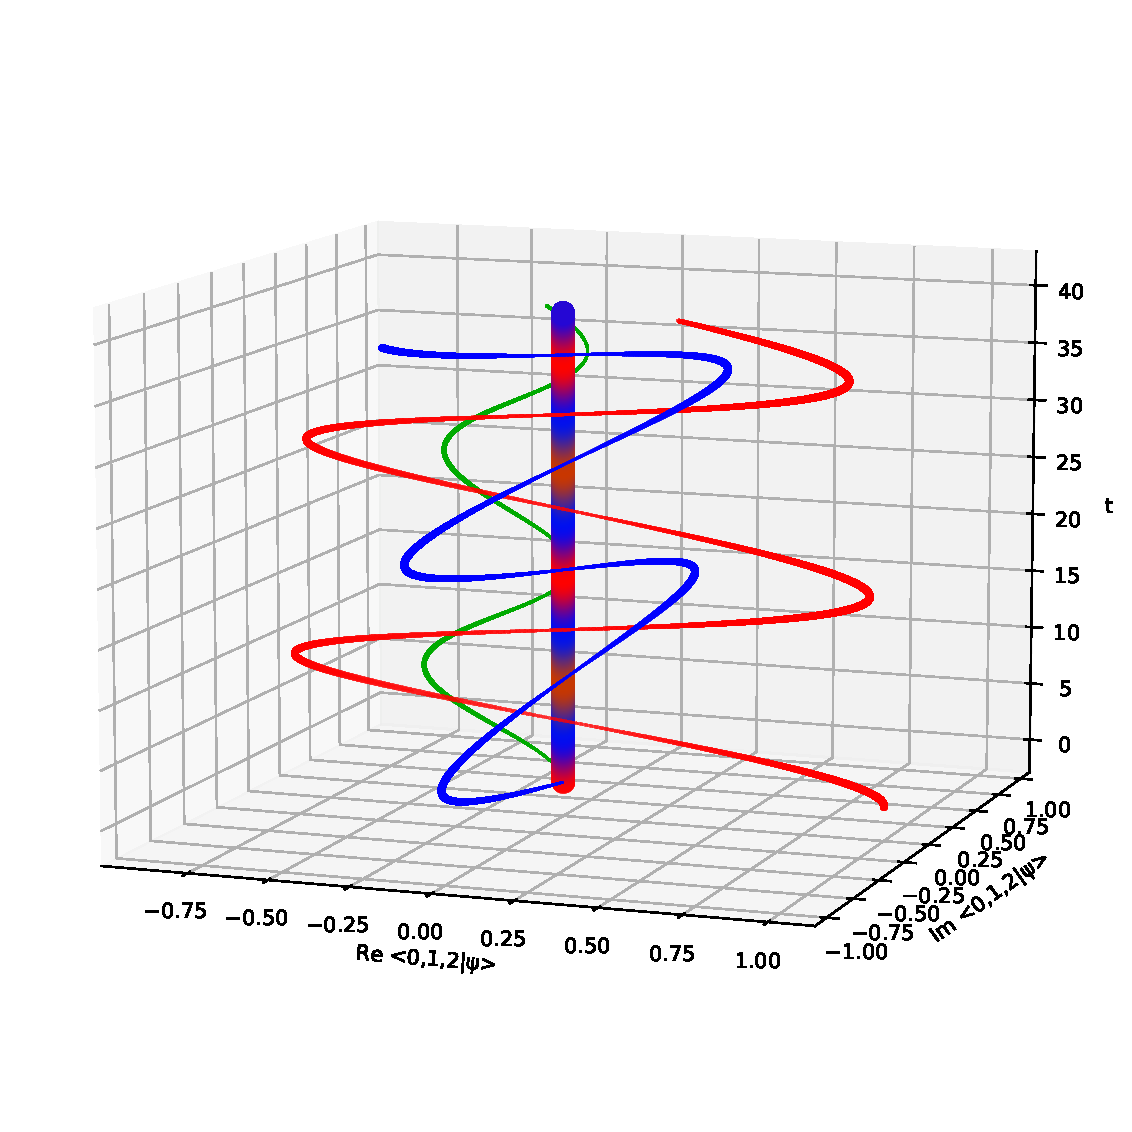
\includegraphics[height=0.45\textheight,clip,trim=80 180 40 140]{img/3ldetect/hermitianSpaceTime_side.pdf}
    \caption{``Side'' view.}
  \end{subfigure}
  \par\bigskip
  \begin{subfigure}[b]{\textwidth}
    \centering
    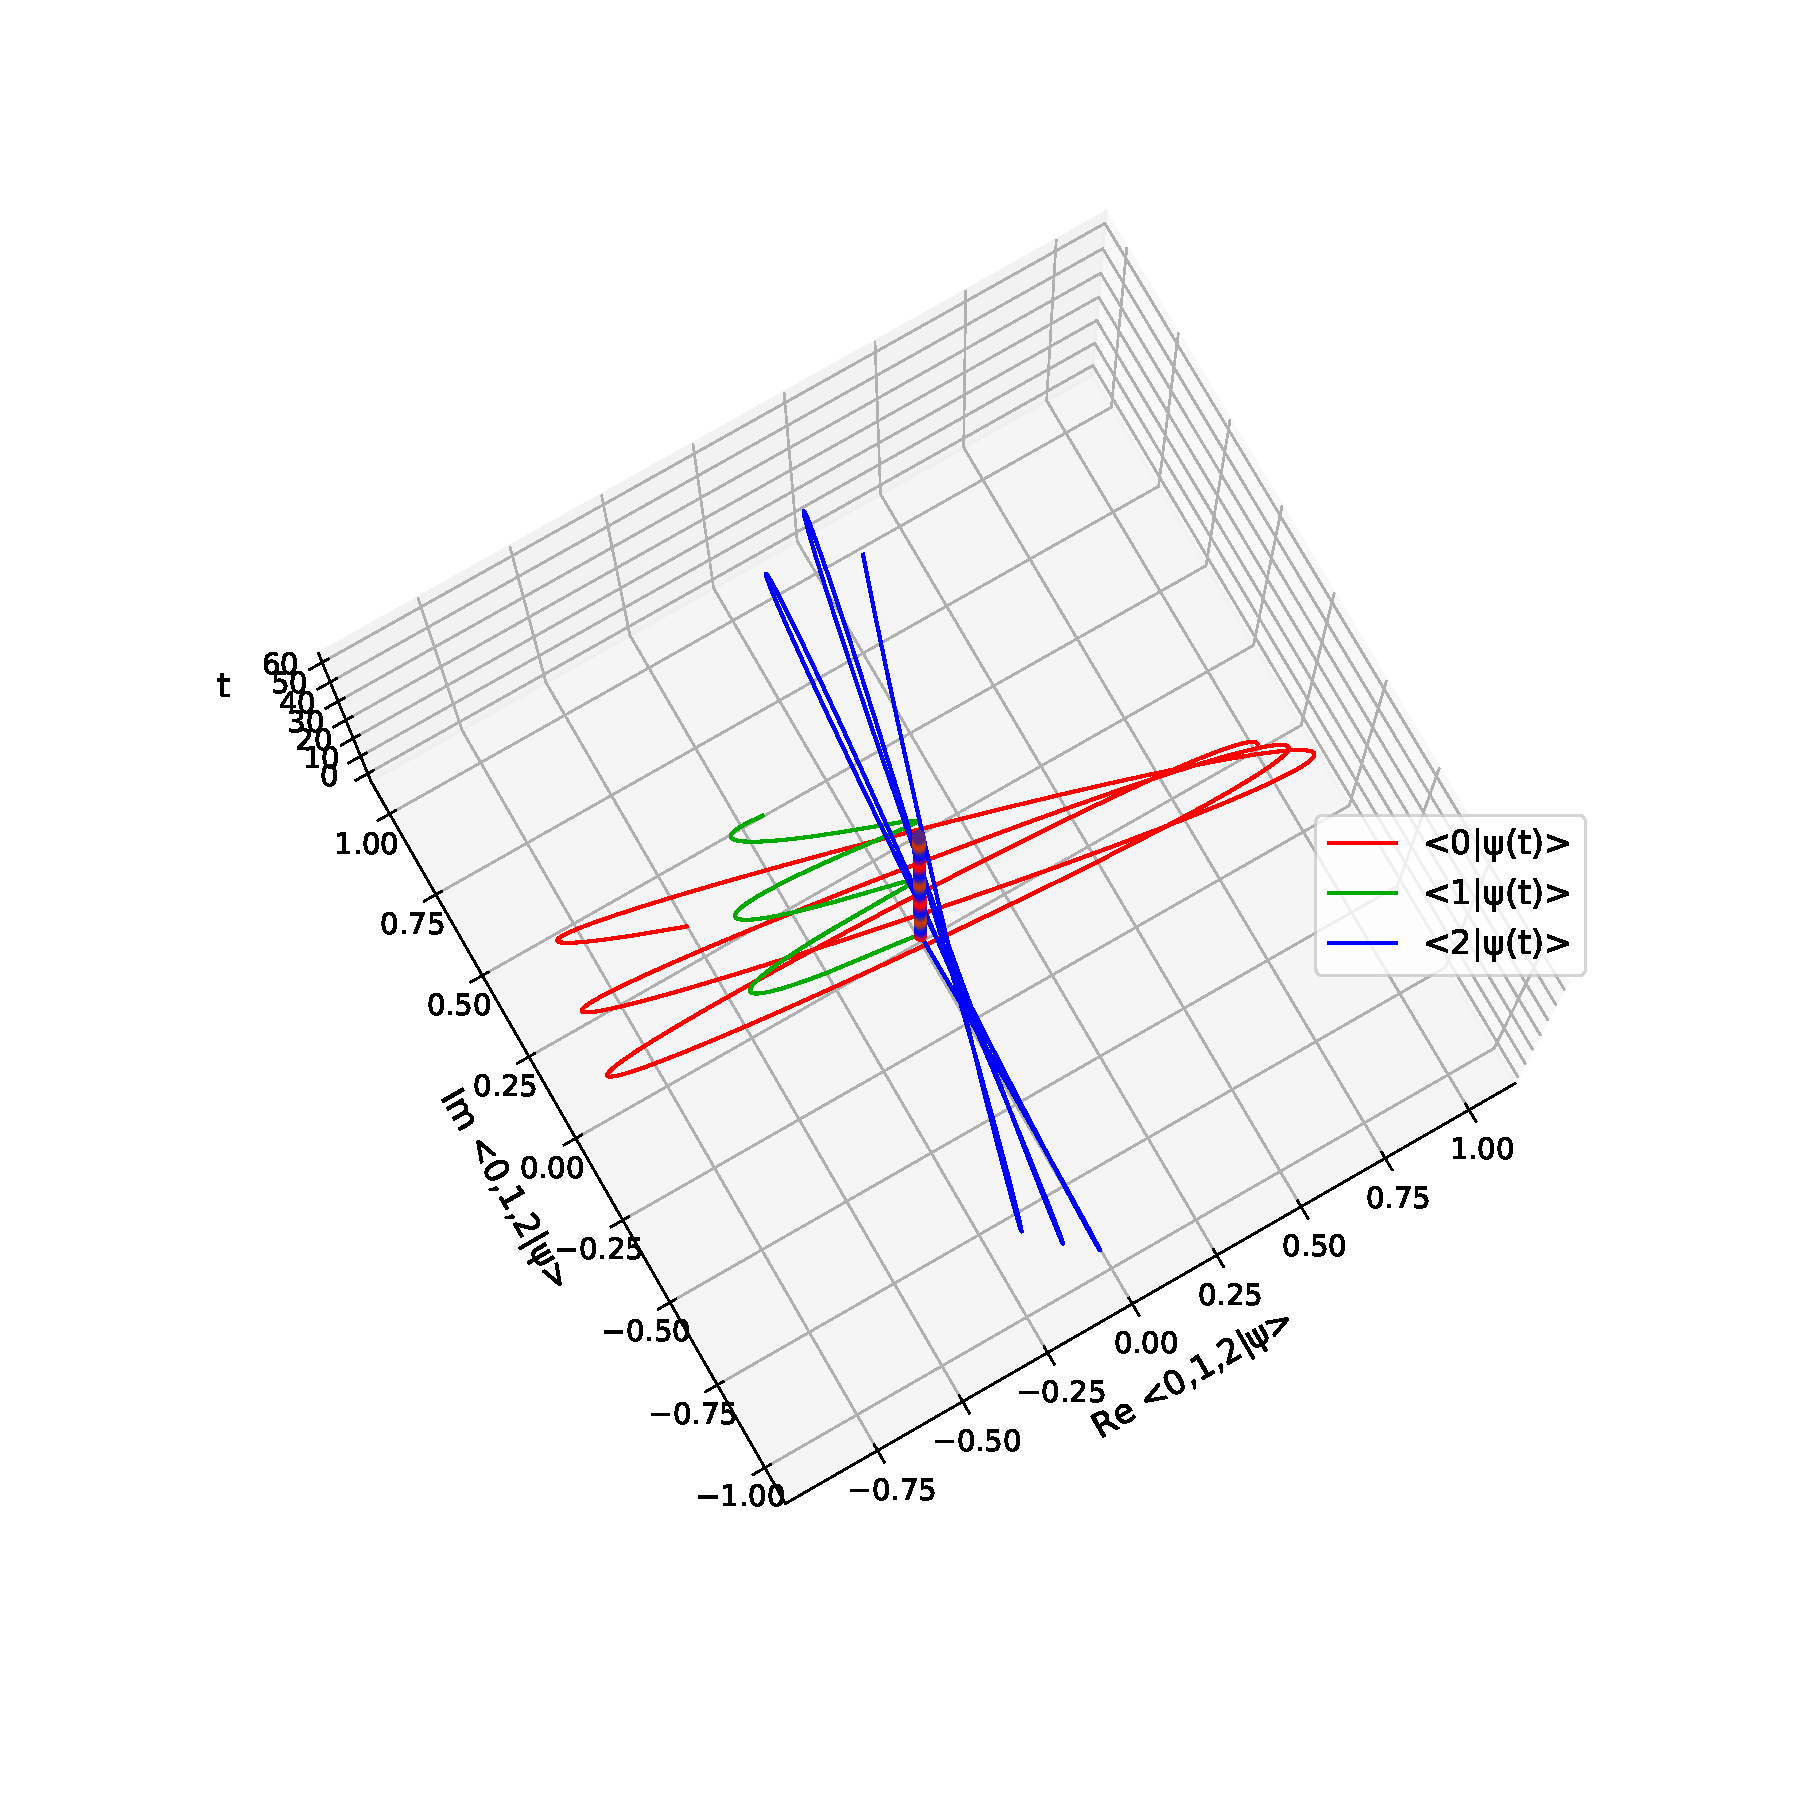
\includegraphics[height=0.41\textheight,clip,trim= 20 120 20 220]{img/3ldetect/hermitianSpaceTime_top.pdf}
    \caption{``Top'' view.}
  \end{subfigure}
  \caption{
    \textit{3-D plot} showing the complex values of the
    probability \emph{amplitudes} $\braket{0, 1, 2}{\psi(t)}$.
    Real and imaginary parts of those values are represented on
    the first two axes, while the independent variable (time, $t$)
    is represented
    on the third axis.
    -- Additionally, the vertical axis is coloured to encode \emph{probabilities}
    (absolute values)
    in a similar fashion to Fig. \ref{fig:3lev:probs:lines}. 
  }
  \label{fig:3lev:hermitianEvol}
\end{figure}

---Other than visualizing complex-valued functions with three-dimensional plots,
another visualization technique, utilized in various plots in this Section,
consists of leveraging
the fact that the system has exactly 3 levels,
thus allowing three primary colors, red, green and blue, to be combined
in proportion to the probabilities $\abs{\braket{i}{\psi(t)}}$
respectively for $i = 0, 1, 2$. This allows an immediate visualization
of which level, $\ket{0}$, $\ket{2}$ or $\ket{2}$, predominates statistically, if any.


%%%%%%%%%%%%%%%%%%%%%%%%%%%%%%%%%%%%%%%%%%%%%%%%%%%%%%%%%%%%%%%%%%%%%%%

%%
%%
%%
%%

% Pobabilities (non-Hermitian) and loss of normalization

\begin{figure}[h]
  \begin{subfigure}[b]{\textwidth}
    \centering
    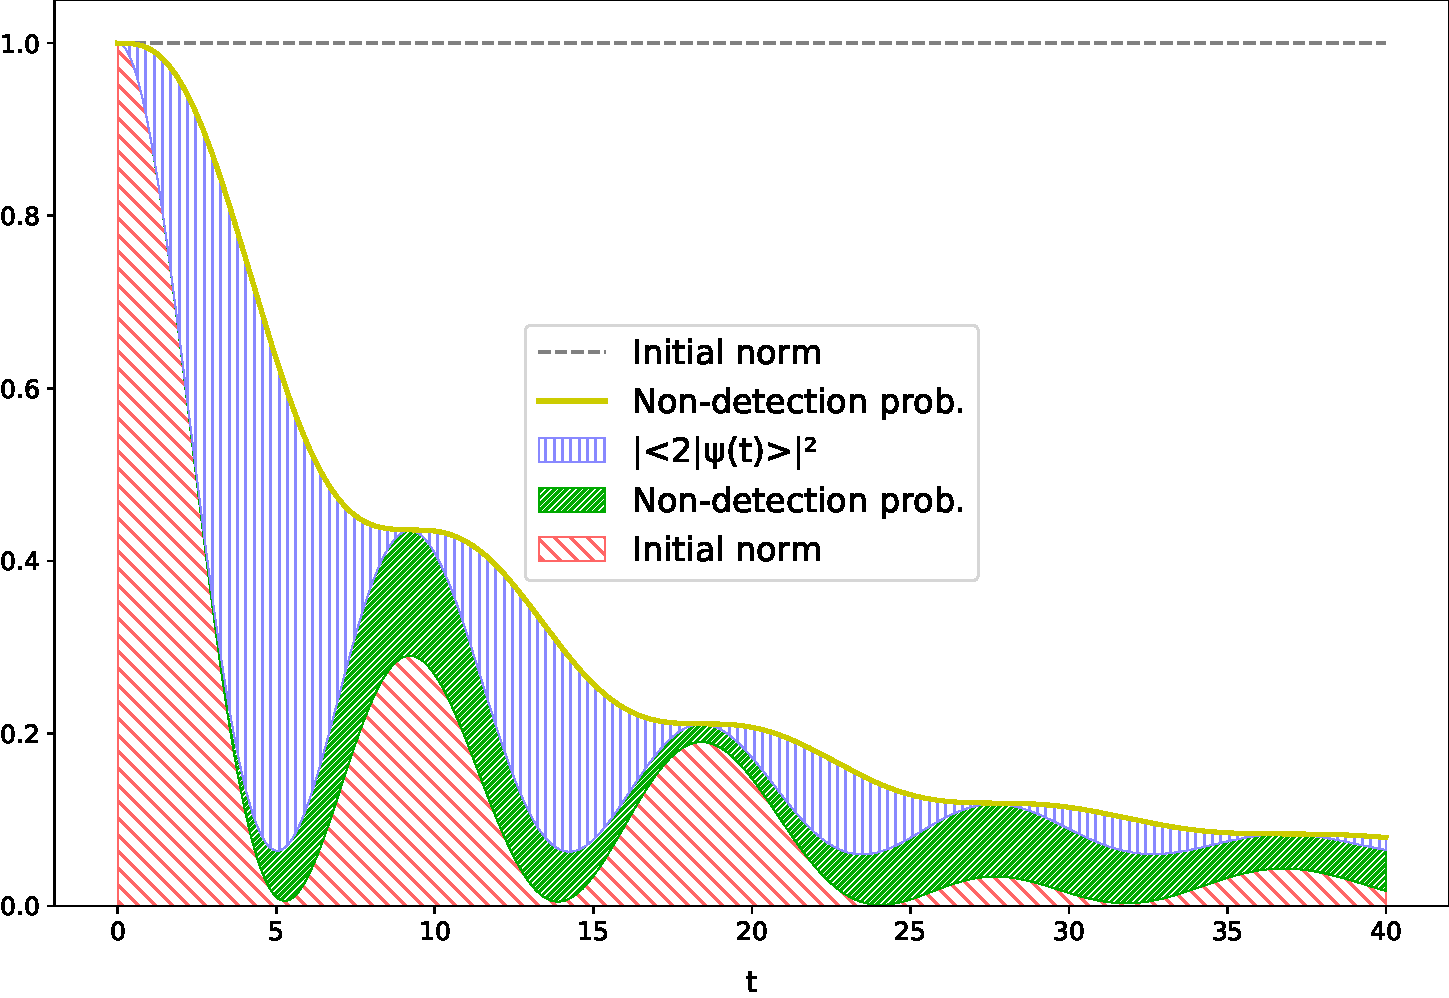
\includegraphics[width=.8\textwidth]{img/3ldetect/loss3color.pdf}
    \subcaption{Foo.}%\label{fig:aabsorbed-qubit-components_pwlattice:re0}
  \end{subfigure}
  \par\bigskip
  \par\bigskip
  \begin{subfigure}[b]{\textwidth}
    \centering
    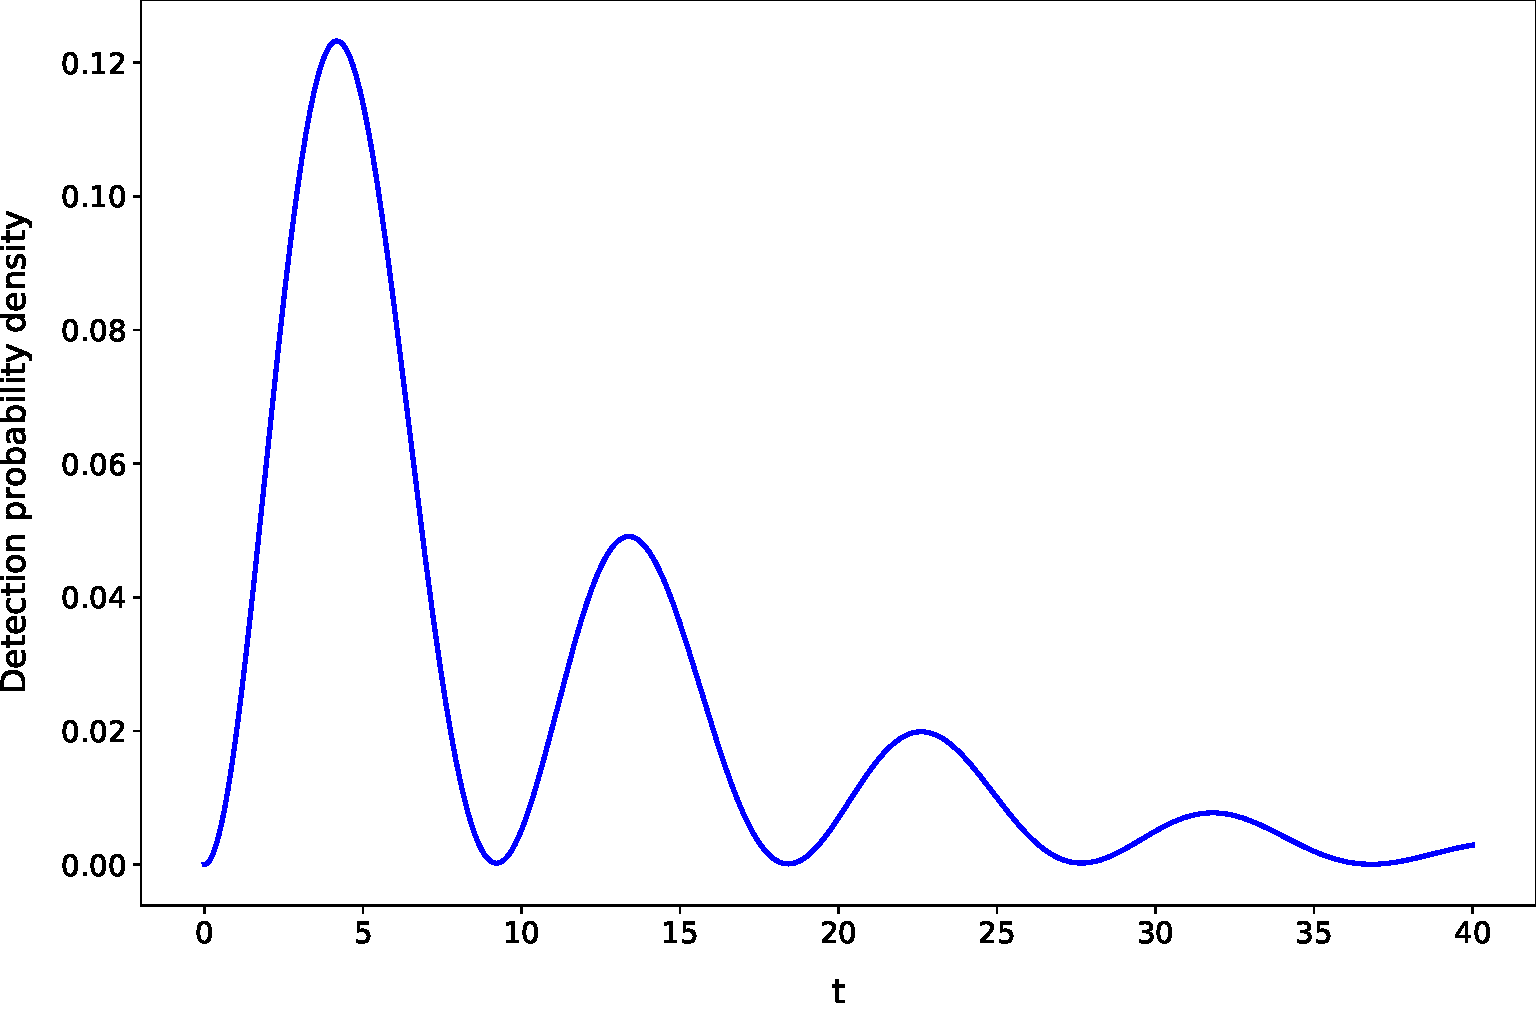
\includegraphics[width=.8\textwidth]{img/3ldetect/loss.pdf}
    \subcaption{Bar.}%\label{fig:aabsorbed-qubit-components_pwlattice:im1}
  \end{subfigure}
  \par\bigskip
  \par\bigskip
  \caption{
    Blah blah blah.
  }
  %\label{fig:aabsorbed-qubit-components_pwlattice}
\end{figure}

% extended time

\begin{figure}[h]
  \begin{subfigure}[b]{\textwidth}
    \centering
    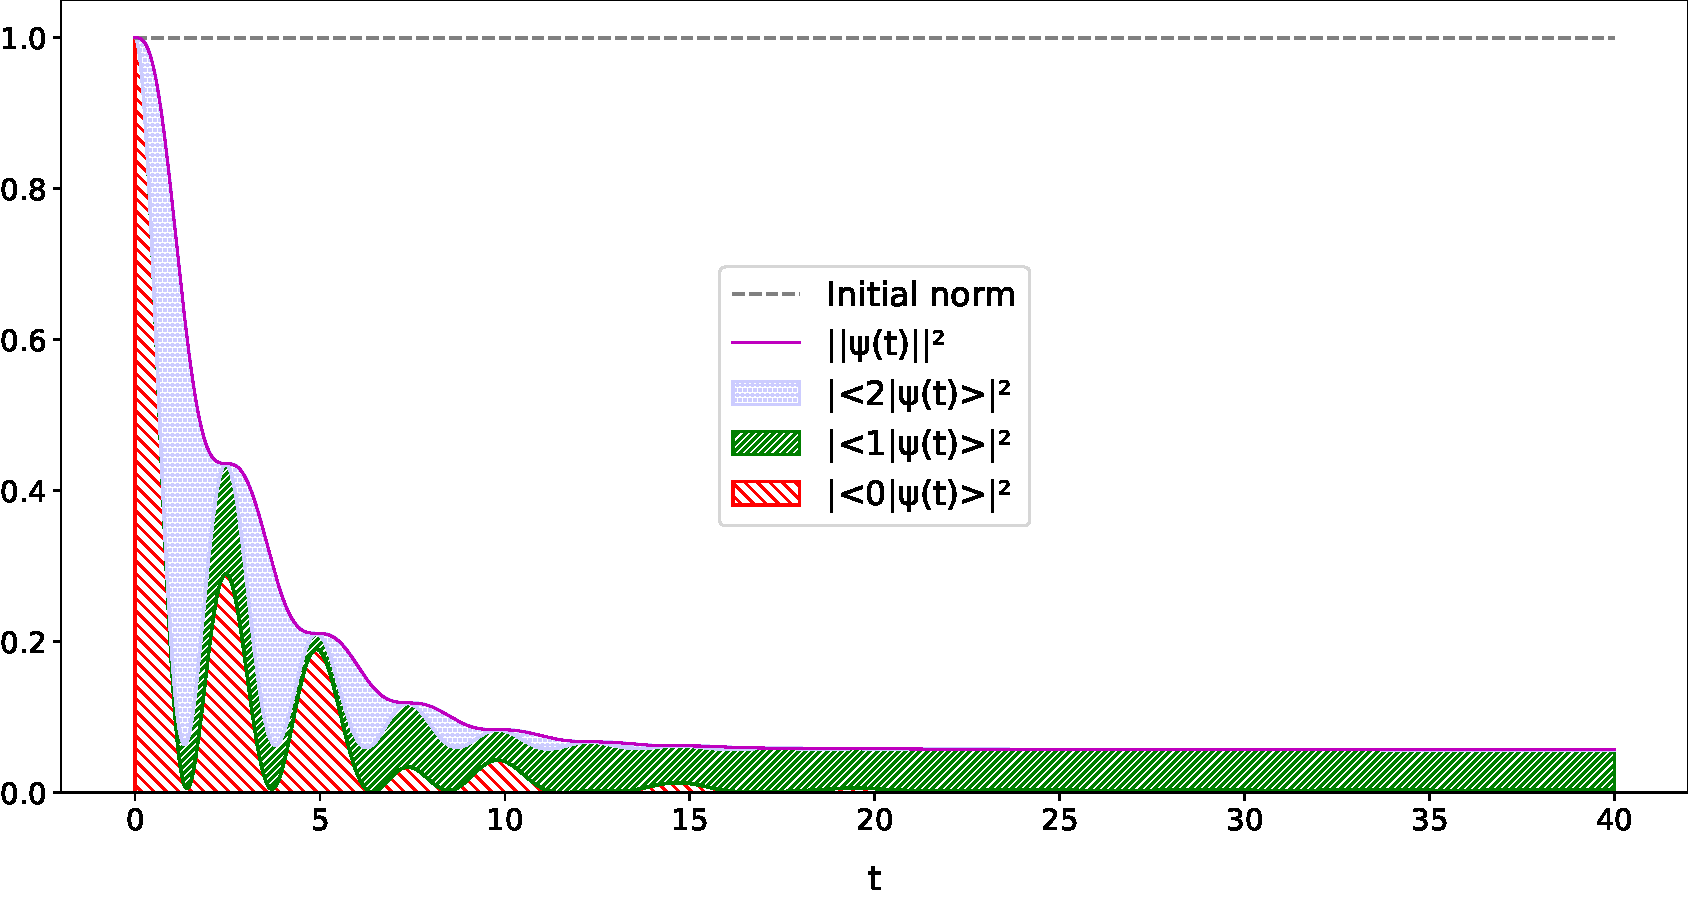
\includegraphics[width=\textwidth]{img/3ldetect/loss3color_ext.pdf}
    \subcaption{Foo.}%\label{fig:aabsorbed-qubit-components_pwlattice:re0}
  \end{subfigure}
  \par\bigskip
  \par\bigskip
  \begin{subfigure}[b]{\textwidth}
    \centering
    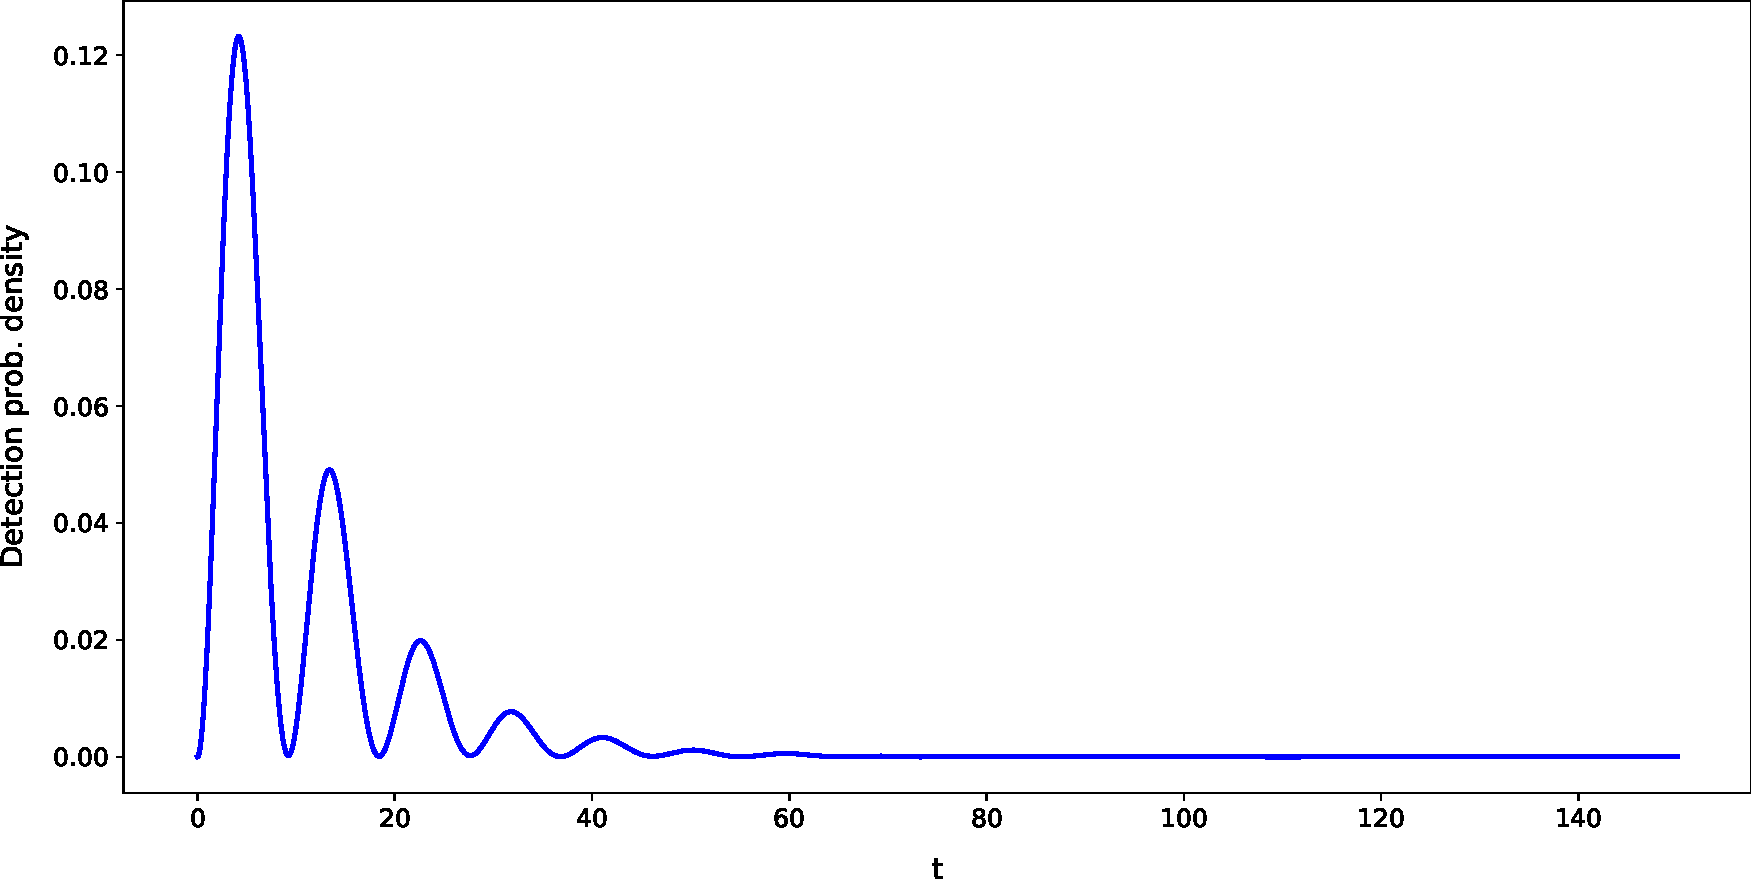
\includegraphics[width=\textwidth]{img/3ldetect/loss_ext.pdf}
    \subcaption{Bar.}%\label{fig:aabsorbed-qubit-components_pwlattice:im1}
  \end{subfigure}
  \par\bigskip
  \par\bigskip
  \caption{
    Blah blah blah.
  }
  %\label{fig:aabsorbed-qubit-components_pwlattice}
\end{figure}

% "3D"

\begin{figure}[h]
  \begin{subfigure}[b]{\textwidth}
    \centering
    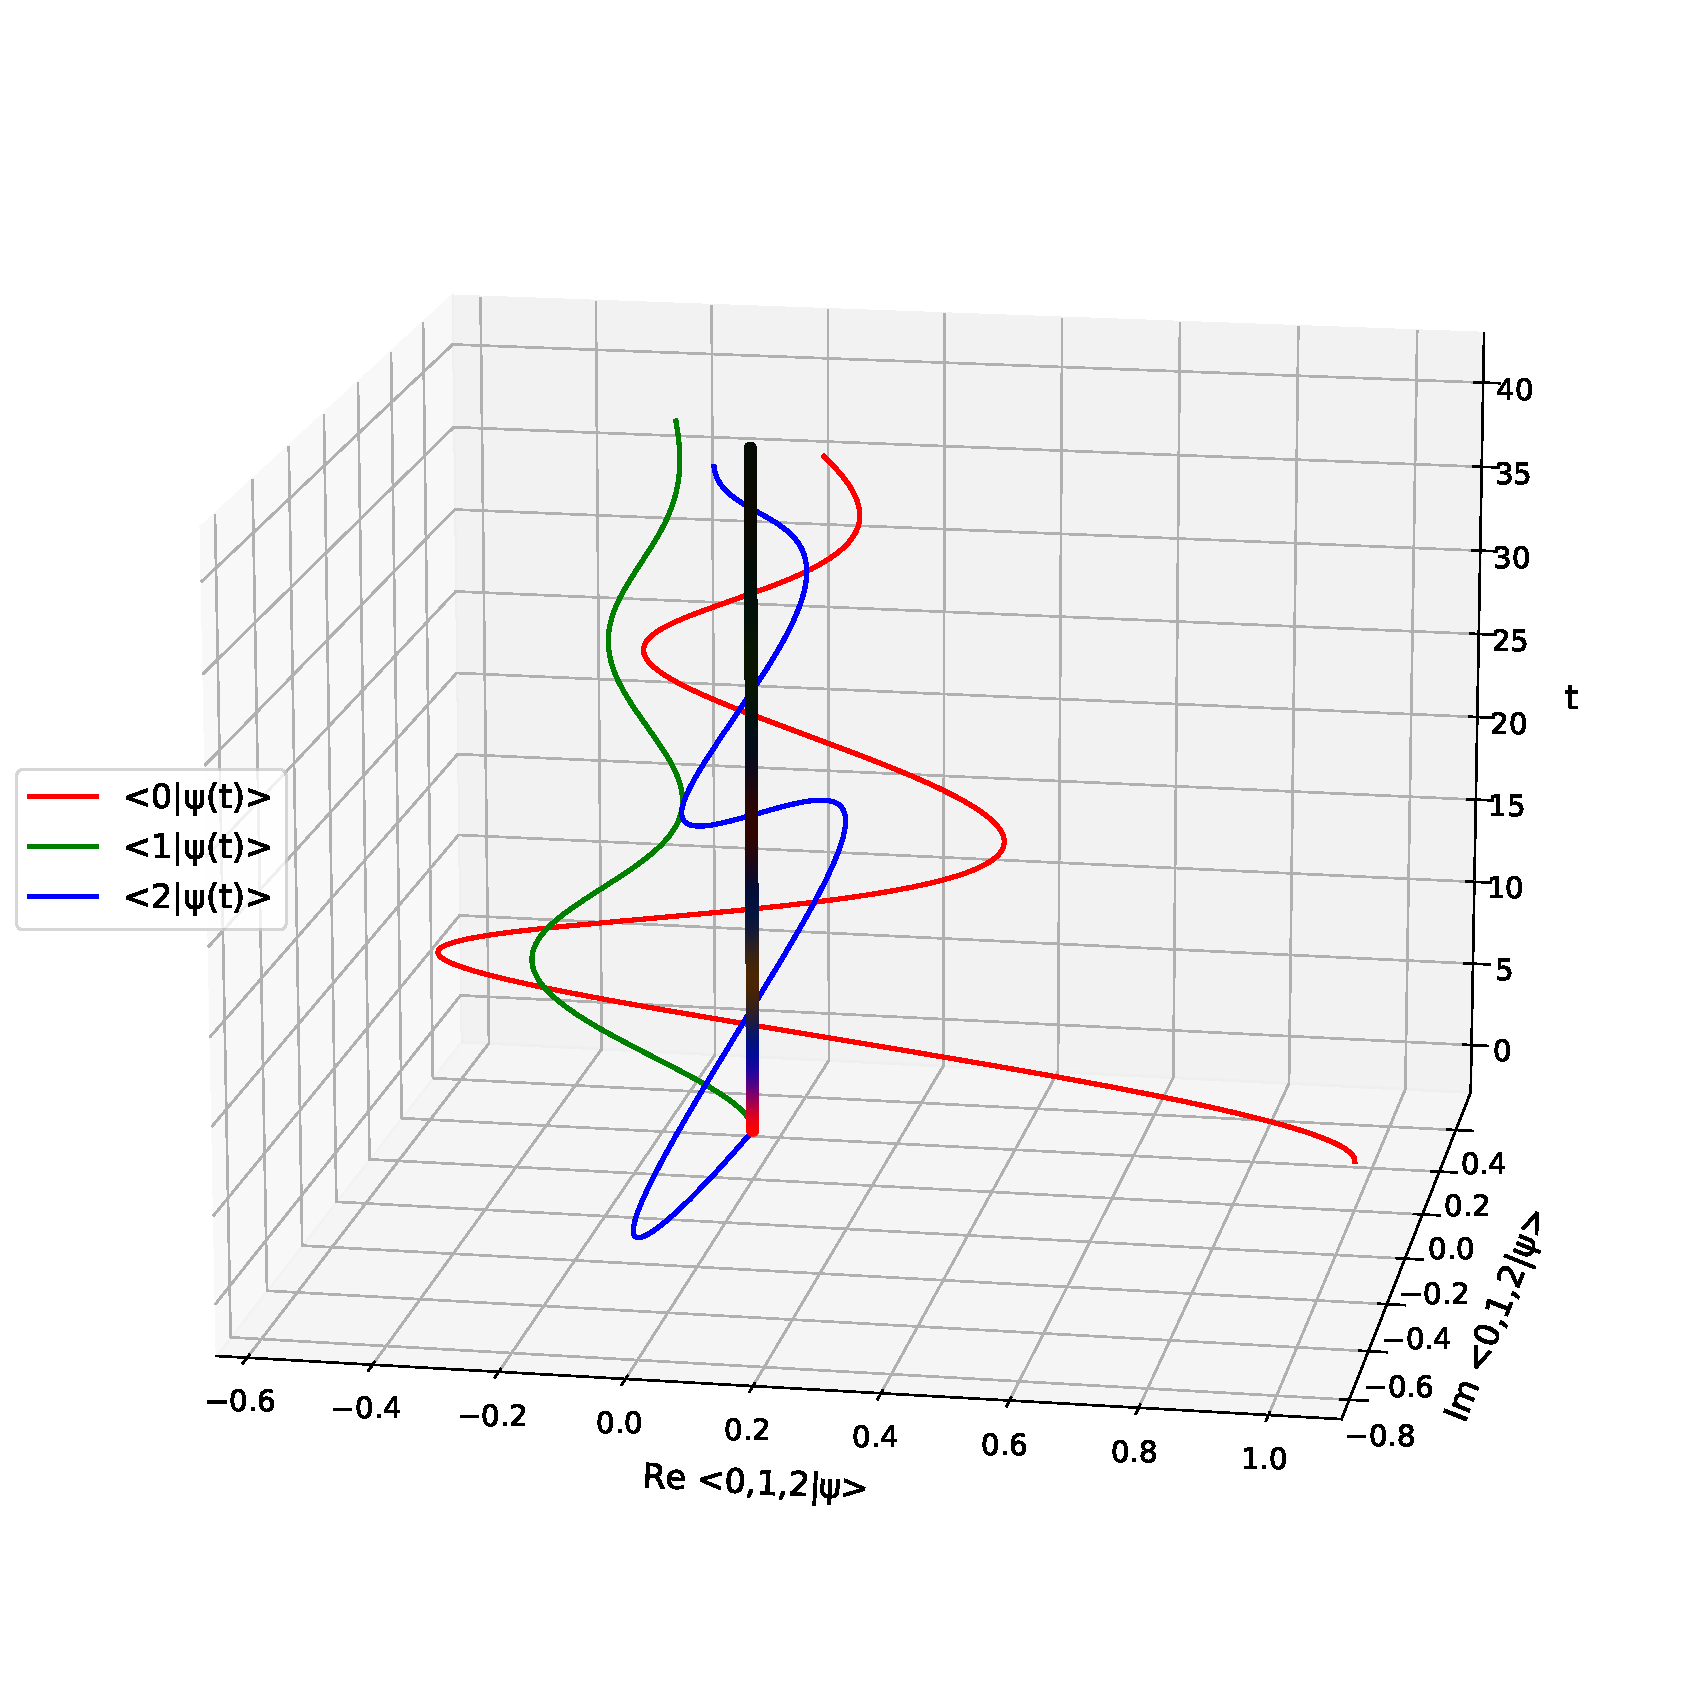
\includegraphics[height=0.41\textheight,clip,trim=0 90 40 140]{img/3ldetect/NonHermitianSpaceTime_side.pdf}
    \caption{Foo.}
  \end{subfigure}
  \par\bigskip
  \begin{subfigure}[b]{\textwidth}
    \centering
    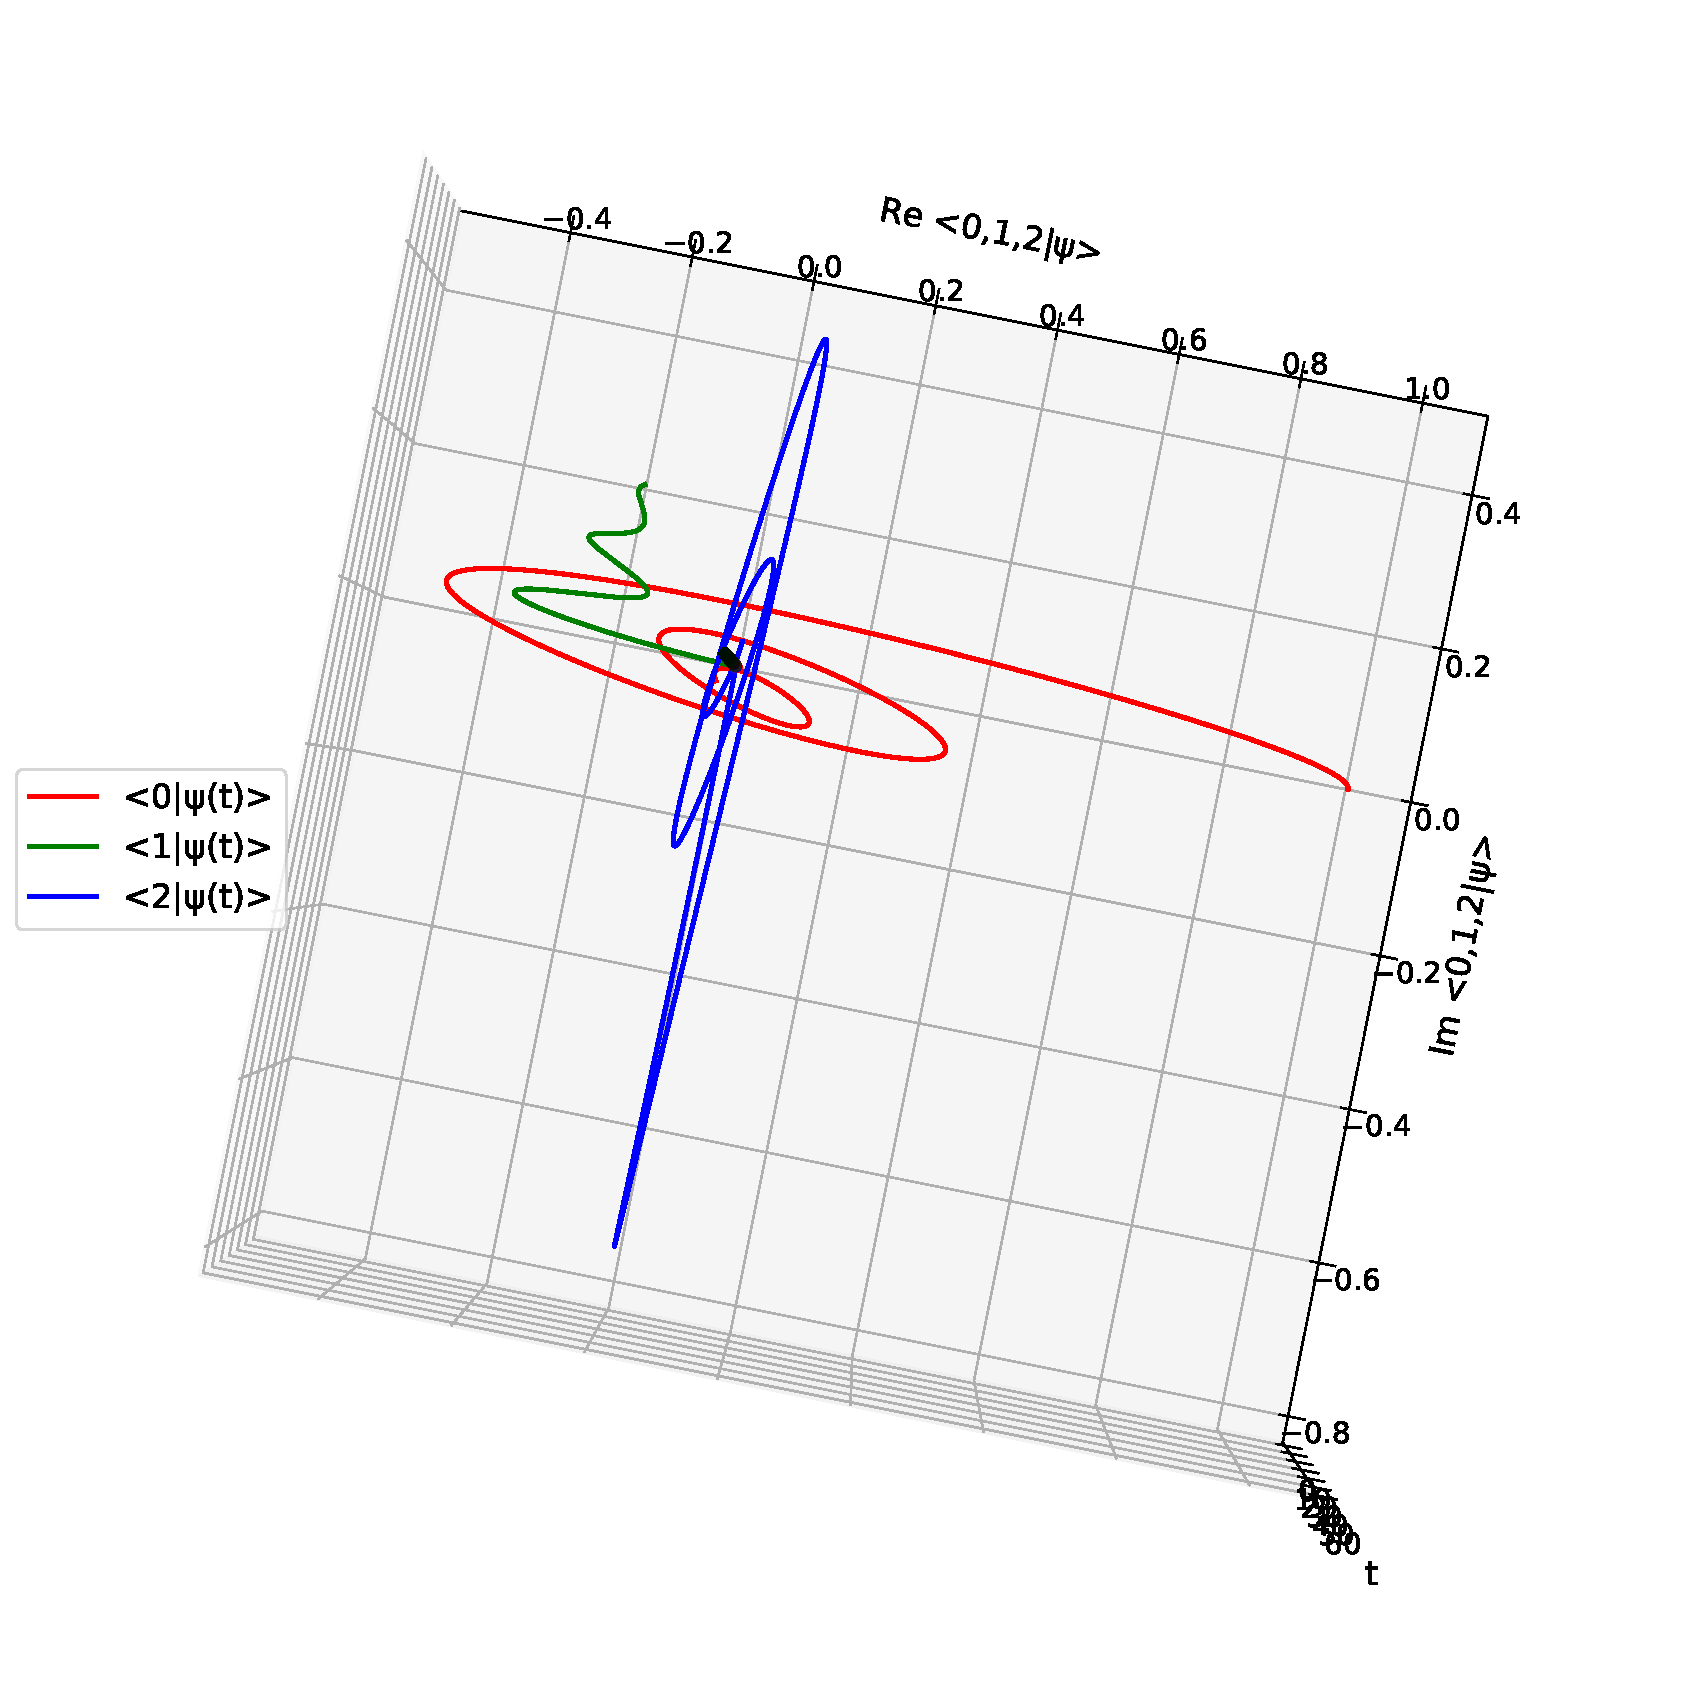
\includegraphics[height=0.44\textheight,clip,trim= 0 90 20 75]{img/3ldetect/NonHermitianSpaceTime_top.pdf}
    \caption{Bar.}
  \end{subfigure}
  \caption{FooBar.}
  %\label{fig:psi_V}
\end{figure}

% P-W

\begin{figure}[h]
  \begin{subfigure}[b]{\textwidth}
    \centering
    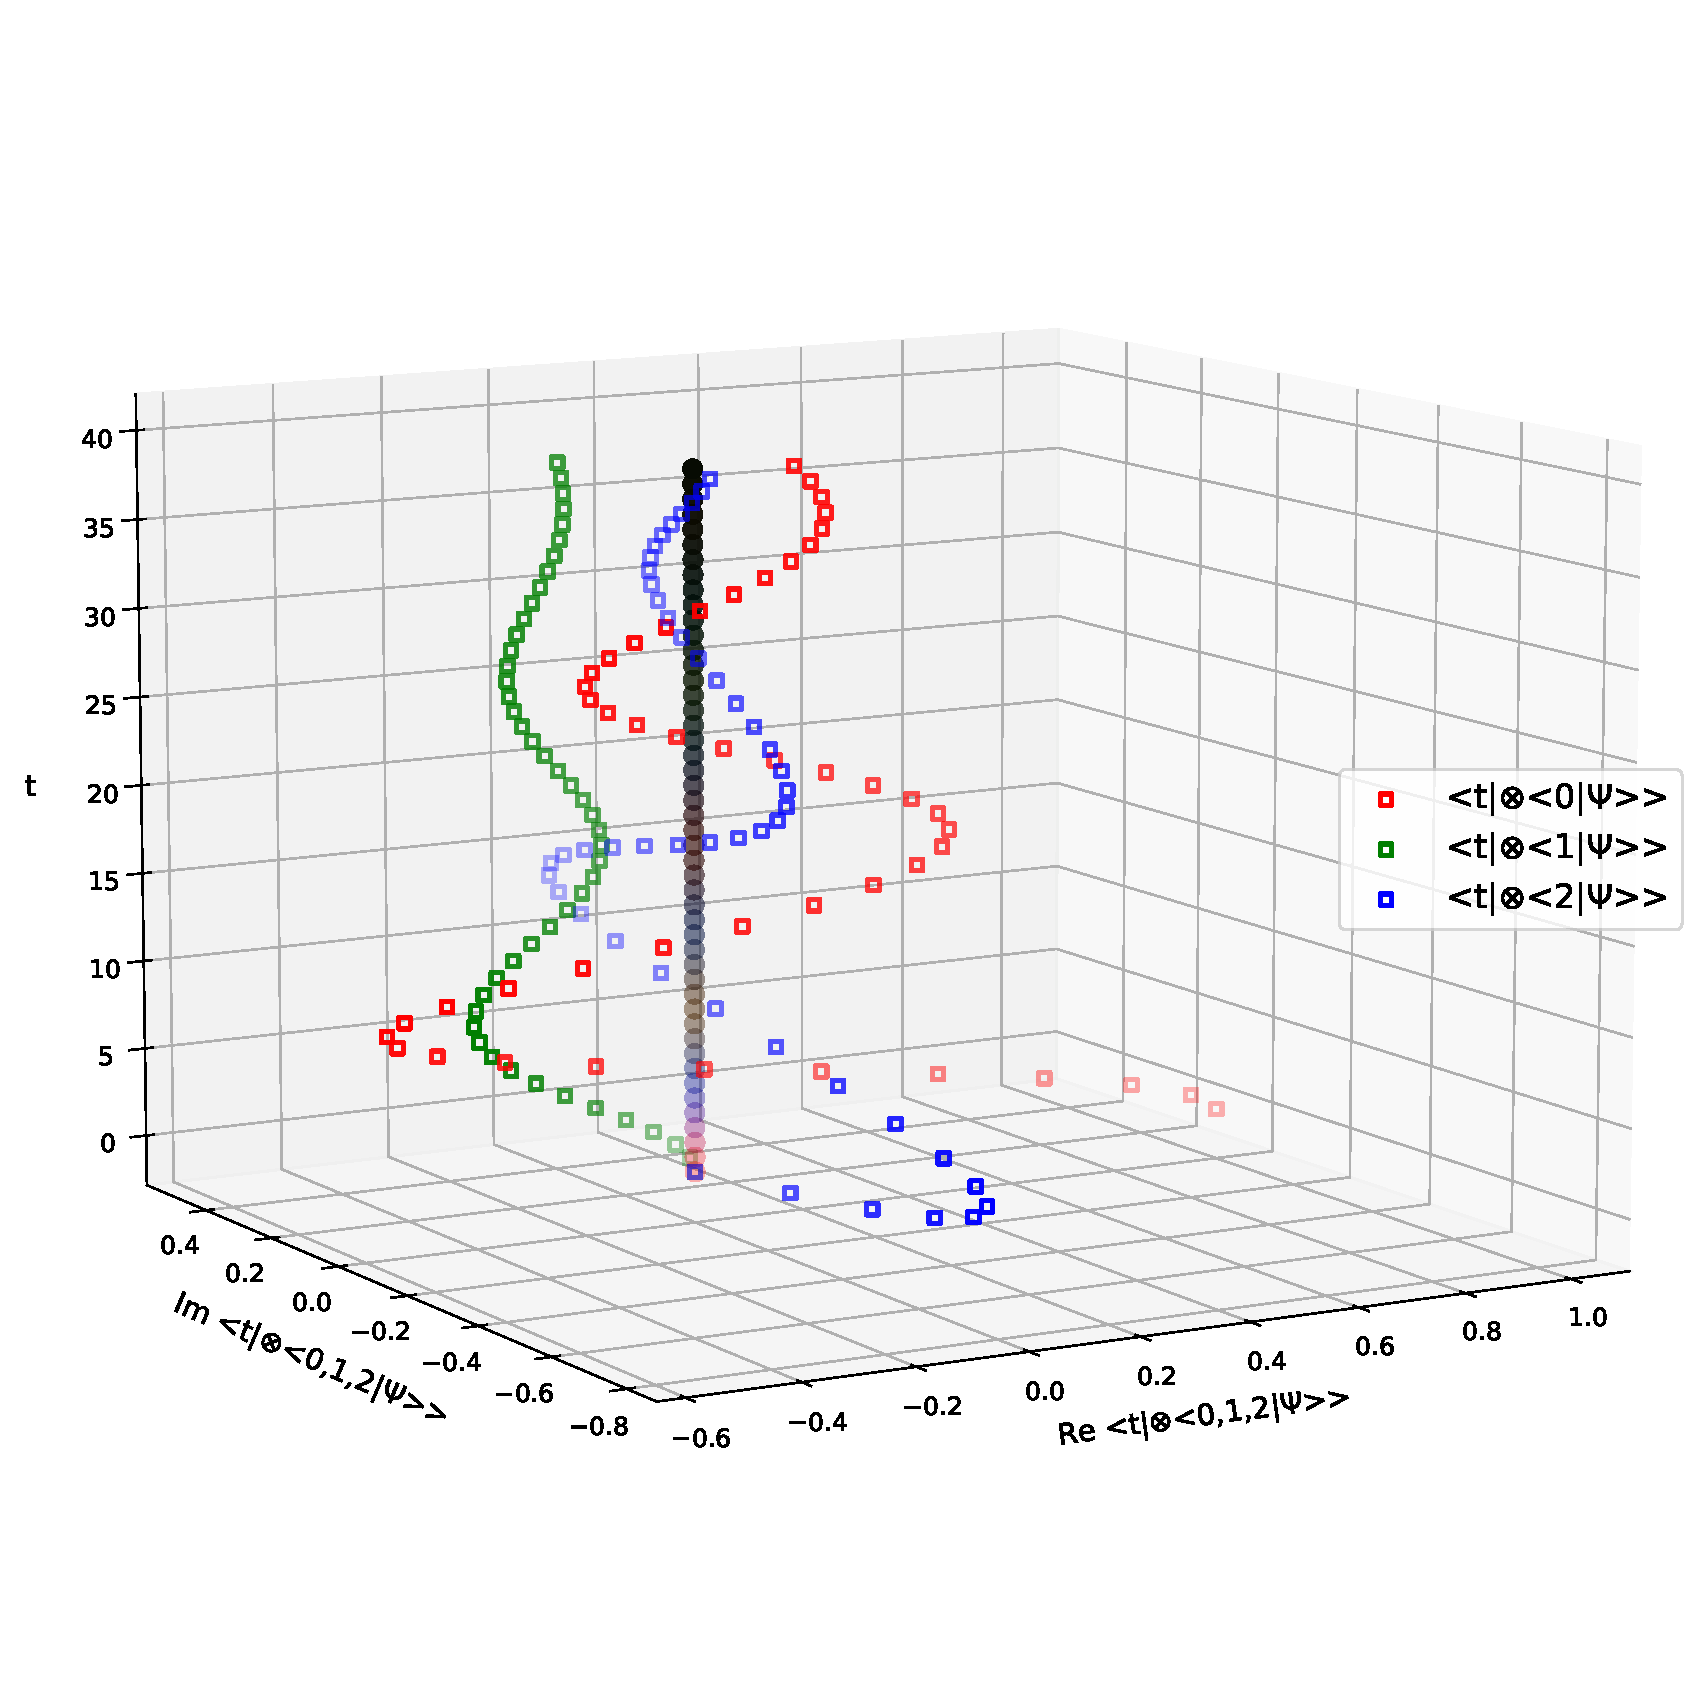
\includegraphics[height=0.41\textheight,clip,trim=0 90 0 140]{img/3ldetect/PWSpaceTime_side.pdf}
    \caption{Foo.}
  \end{subfigure}
  \par\bigskip
  \begin{subfigure}[b]{\textwidth}
    \centering
    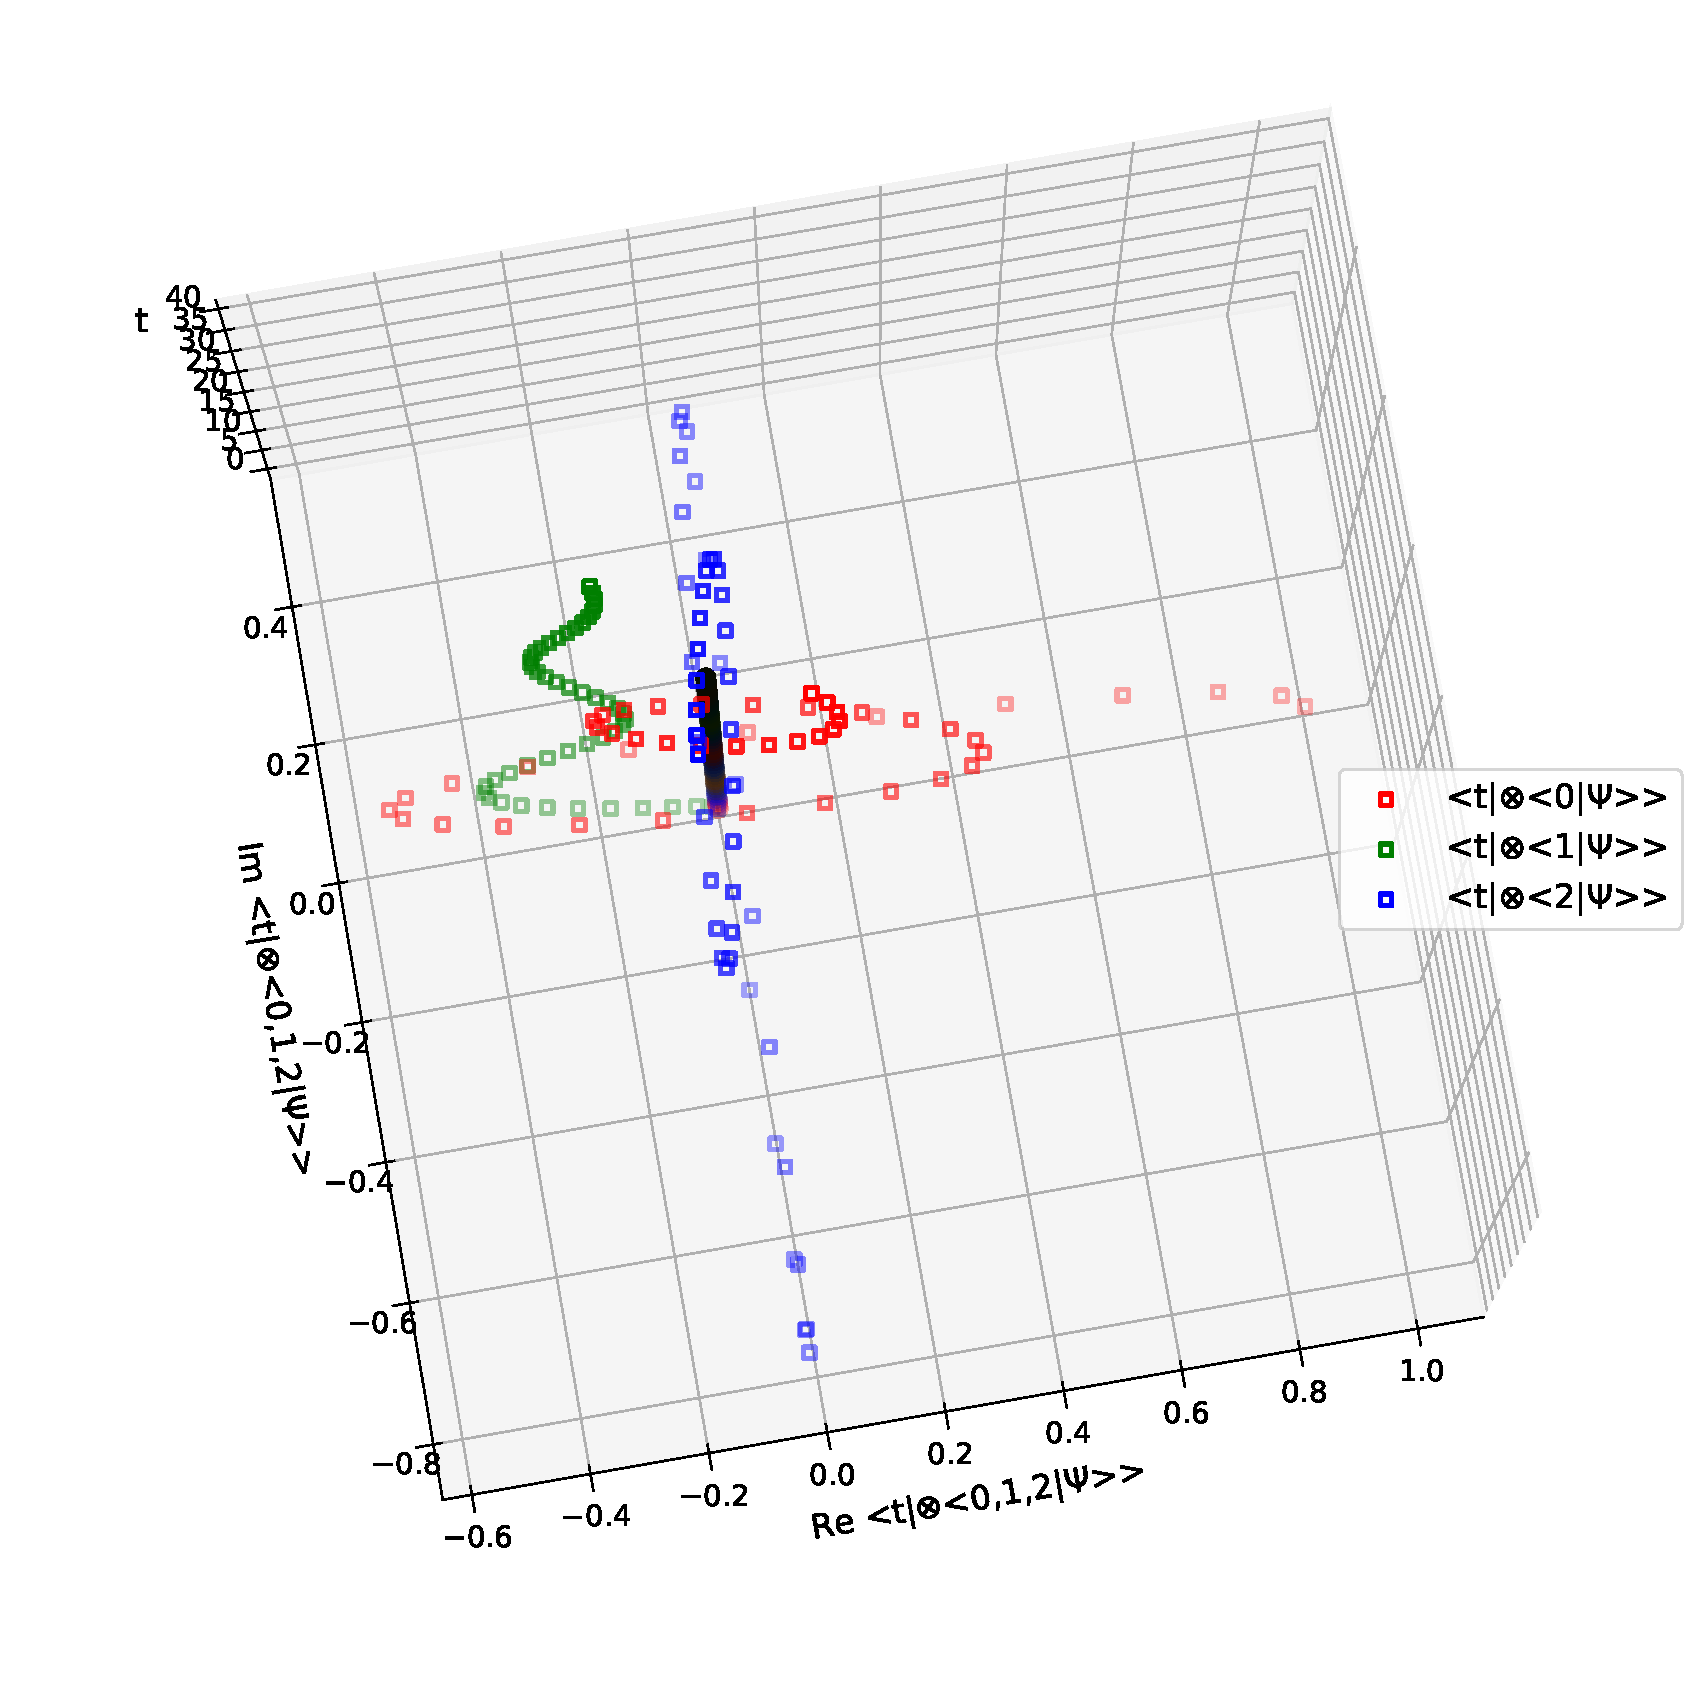
\includegraphics[height=0.48\textheight,clip,trim= 0 60 0 100]{img/3ldetect/PWSpaceTime_top.pdf}
    \caption{Bar.}
  \end{subfigure}
  \caption{FooBar.}
  %\label{fig:psi_V}
\end{figure}

% P-W vs QM


\begin{figure}[h!]
  \cleardoublepage
  \centering
  \begin{subfigure}{\textwidth}
      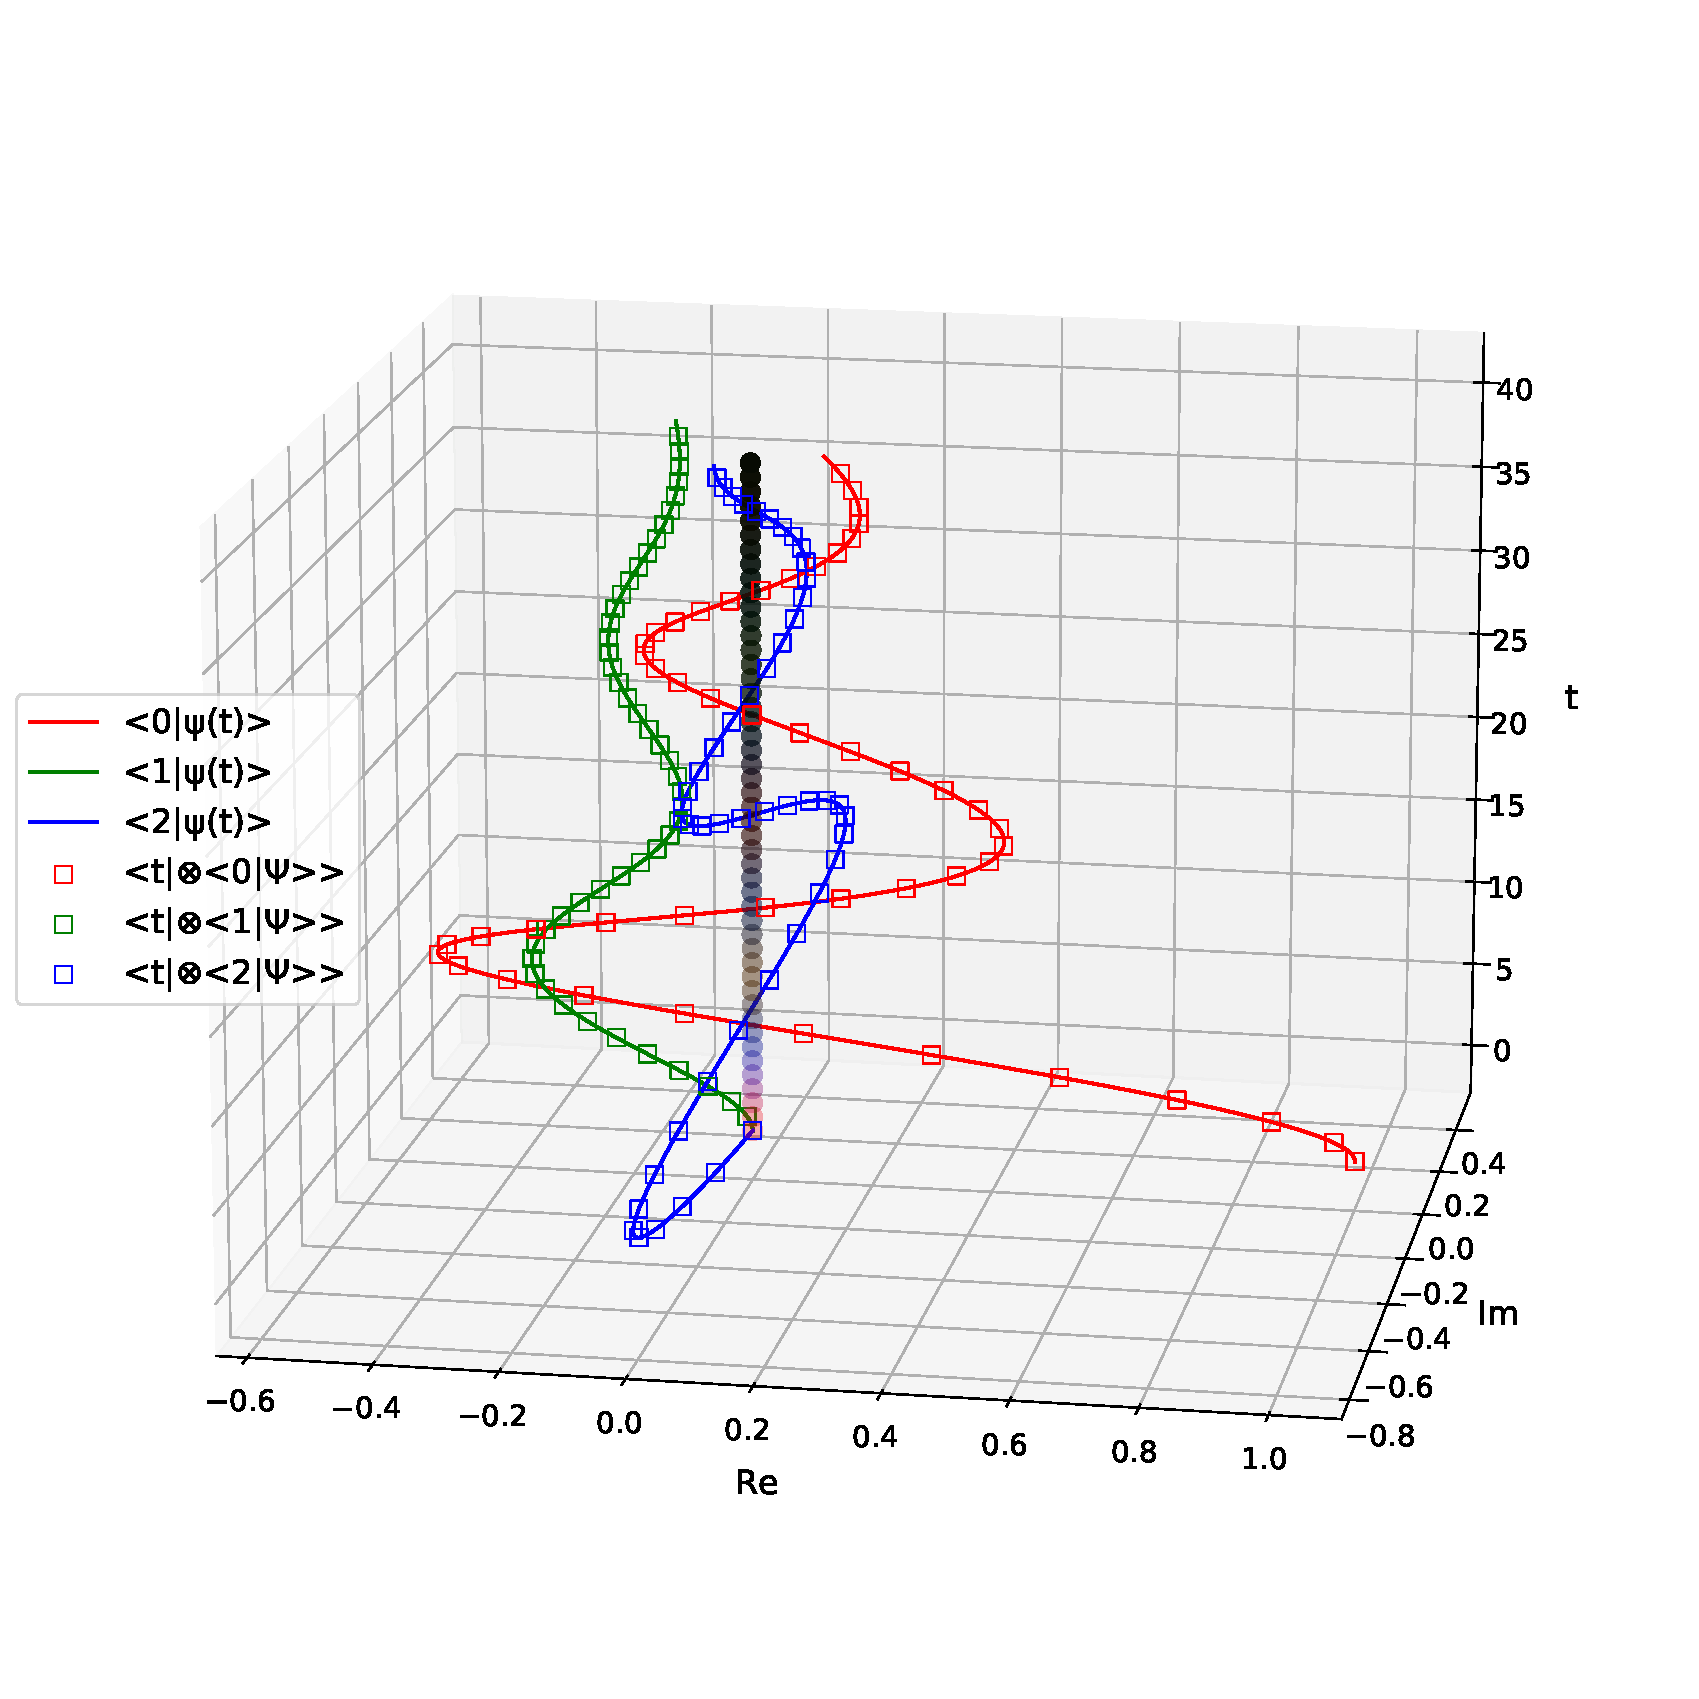
\includegraphics[width=\textwidth]{img/3ldetect/PWSpaceTimeFit_side.pdf}
      \subcaption{Foo.}
      %\label{fig:arm1}
  \end{subfigure}
  \caption{Foobar.}
\end{figure}
\begin{figure}\ContinuedFloat
  \centering
  \begin{subfigure}{\textwidth}
      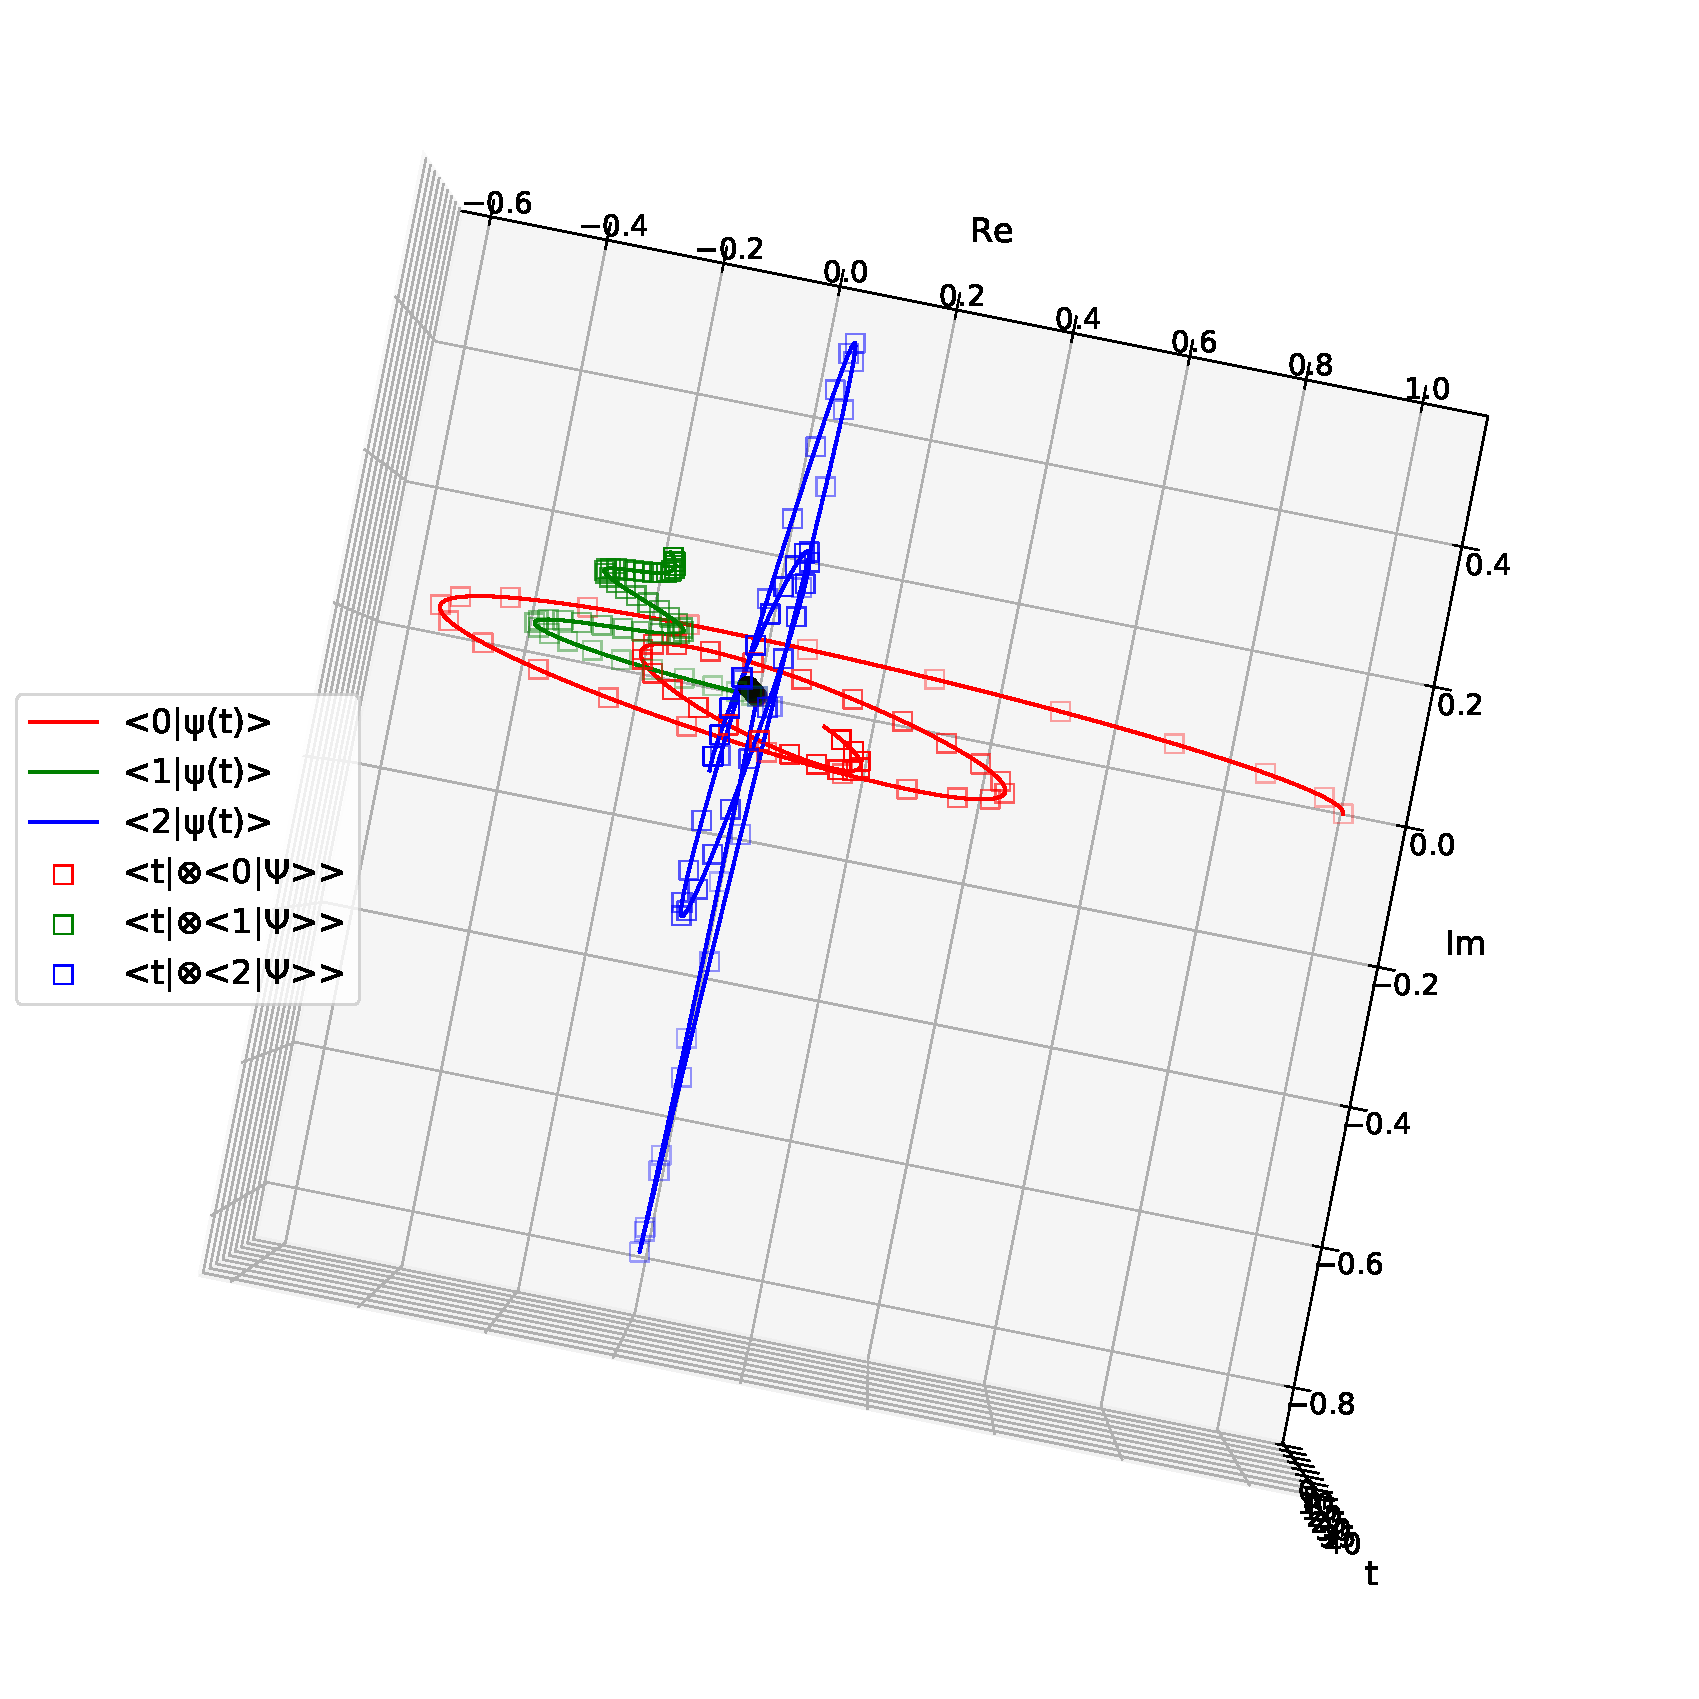
\includegraphics[width=\textwidth]{img/3ldetect/PWSpaceTimeFit_top.pdf}
      \subcaption{Bar.}
      %\label{fig:arm3}
  \end{subfigure}
  \caption{Foobar (cont.)}
\end{figure}

% P-W (bayesian) vs Detector model (norm. loss, Allcock...) detection probability

\begin{figure}[h!]
  \centering
  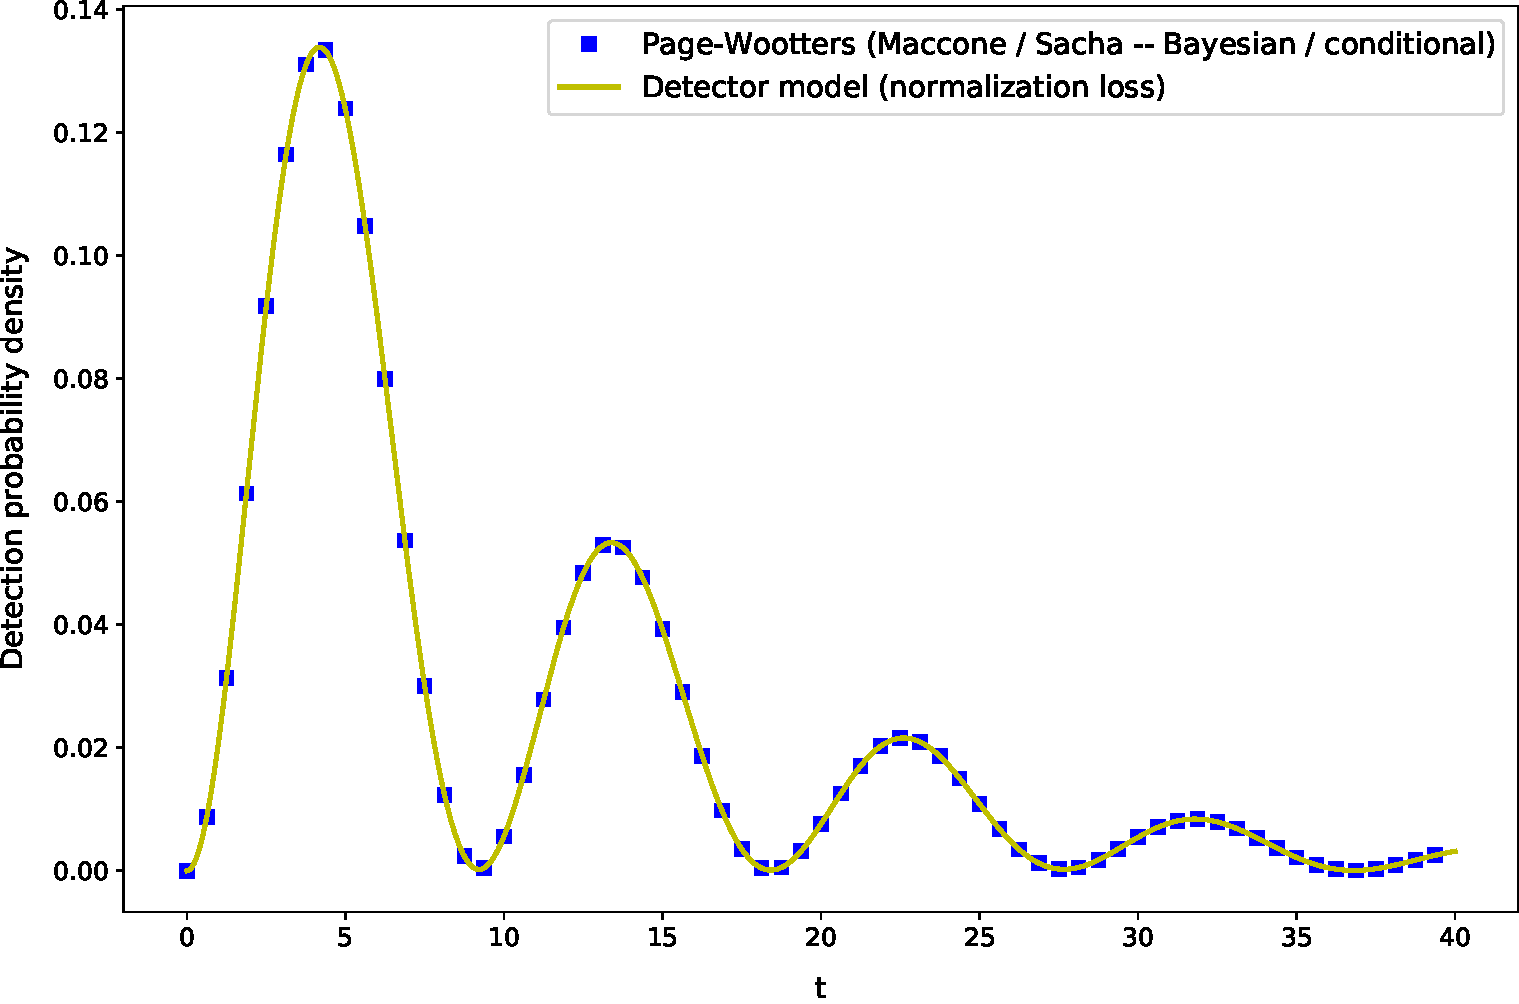
\includegraphics[width=\textwidth]{img/3ldetect/conditionalProbFit.pdf}
  \caption{Foo.}
  %\label{fig:psi_V}
\end{figure}